\documentclass[a4paper,12pt]{article}
\usepackage[fleqn]{amsmath}
\usepackage{amssymb}
\usepackage{graphicx}
\graphicspath{ {./images/} }
\newcommand\longdiv[2]{%
$\strut#1$\kern.25em\smash{\raise.3ex\hbox{$\big)$}}$\mkern-8mu
        \overline{\enspace\strut#2}$}
\begin{document}

\title{Polynomials}	
\author{Edward Jex}
\maketitle

The order / degree of a polynomial is the highest power of the variable it contains. For example, a polynomial is order 3. \\
\section*{Division}
Long division is the best method when it is not known if there is a remainder or not. Otherwise it can  be done by inspection. \\
\subsection*{Example 1}
Divide $2x^3 -3x^2 + x -6$ by $x-2$ \\\\
\phantom{A}\hspace{0.8cm} $2x^2 + x + 3$ \\
\longdiv{x-2}{2x^3 -3x^2 + x -6} \\
\phantom{A}\hspace{0.3cm} $-(2x^3 -4x^2)$ \\
\phantom{A}\hspace{2.1cm} $x^2$ \\
\phantom{A}\hspace{1.6cm} $-(x^2-2x)$ \\
\phantom{A}\hspace{3cm} $3x-6$ \\
\phantom{A}\hspace{2.5cm} $-(3x-6)$ \\
\phantom{A}\hspace{4cm} $0$ \\\\
$\Rightarrow 2x^3 -3x^2 + x -6 = (2x^2 + x + 3)(x-2)$
\section*{The Factor Theorem}
We can use the factor theorem to help us to solve algebraic equations of order greater than 2. \\
The factor theorem is as follows: \\
If $(x-\alpha)$ is a factor of $f(x)$ then $f(\alpha) = 0$ and $\alpha$ is the root of the equation of $f(x) = 0$. \\
\subsection*{Example 2}
Show that $(x-1)$ is a linear factor of $2x^3 - 5x^2 - 6x + 9$ \\ 
\begin{align*}
f(1) = 0 & \Rightarrow (x-1) \text{is a factor by the factor theorum} \\
2x^3 - 5x^2 - 6x + 9 & = (x-1)(2x^2-3x-9) \\
& = (x-1)(2x+3)(x-3) \\
& \Rightarrow x = 1, -\frac{3}{2}, 3 \\
\end{align*}
\section*{Sketching Polynomials}
To sketch polynomials, we must find where it crosses the x-axis and y-axis. We also need to know what order the polynomial is so that we know the general shape.  \\
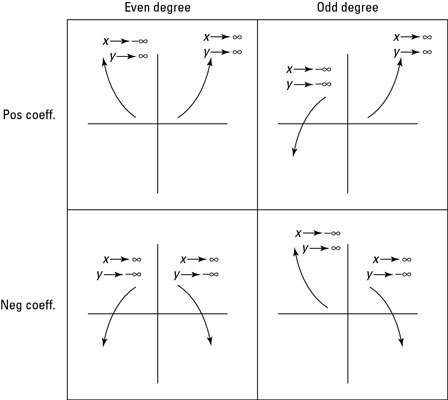
\includegraphics[scale=0.7]{Graphs}
\subsection*{Turning Points}
A point where the gradient is 0. If a polynomial is of order n, it can at most n-1 turning points. 

\section*{Roots of Polynomials}
We denote the root of polynomials using Greek letters starting from $\alpha$.
\subsection*{Notation}
We write:
\begin{align*}
\sum \alpha & = \alpha + \beta + \gamma \\
\sum \alpha \beta & = \alpha \beta + \beta \gamma + \gamma \alpha \\
\sum \alpha^2 \beta & = \alpha^2 \beta + \beta^2 \alpha + \alpha^2 \gamma + \gamma^2 \alpha + \gamma^2 \beta + \beta^2 \gamma \\
\end{align*}
\subsection*{Cubics}
The general equation of a cubic can be written $ax^3 + bx^2 + cx + d = 0 \Rightarrow x^3 + \frac{b}{a}x^2 + \frac{c}{a}x + \frac{d}{a} = 0$, $a \neq 0$. If we know the roots $\alpha$, $\beta$, $\gamma$ it can also be written $(x-\alpha)(x-\beta)(x-\gamma)=0$. If this is expanded we get  $x^3 - (\alpha + \beta + \gamma)x^2 + (\alpha \beta + \beta \gamma + \gamma \alpha)x - \alpha \beta \gamma$. Therefore:
\begin{align*}
\sum \alpha & = \frac{-b}{a} \\
\sum \alpha \beta & = \frac{c}{a} \\
\alpha \beta \gamma & = \frac{-d}{a} \\
\end{align*}
From this we can find the coefficients given information about the roots. 

\subsection*{Quartics}
The general equation of a quartic can be written $x^4 + \frac{b}{a} x^3 + \frac{c}{a} x^2 + \frac{d}{a} x + \frac{3}{a} = 0$ with roots $\alpha$, $\beta$, $\gamma$, $\delta$. As before, it can also be expressed in the form $(x-\alpha)(x-\beta)(x-\gamma)(x-\delta)=0$. Therefore, we get that:
\begin{align*}
\sum \alpha & = \frac{-b}{a} \\
\sum \alpha \beta & = \frac{c}{a} \\
\sum \alpha \beta \gamma & = \frac{-d}{a} \\
\alpha \beta \gamma \delta & = \frac{c}{a} \\
\end{align*}

\subsection*{Related Roots}
If you are given equations for the roots in terms of the roots of a different polynomial you can substitute them in to find the new polynomial. \\

\subsubsection*{Example 1}
$5x^3 - x^2 + 4x + 1 = 0$ has roots $\alpha$, $\beta$, $\gamma$. Find a cubic with the roots $2 \alpha + 3$, $2 \beta + 3$, $2 \gamma + 3$. \\

\begin{align*}
y & = 2x+3 \\
\Rightarrow x & = \frac{y-3}{2} \\
\end{align*}
\begin{align*}
5(\frac{y-3}{2})^3 - (\frac{y-3}{2})^2 + 4(\frac{y-3}{2}) + 1 & = 0 \\
5(y-3)^3 - 2(y-3)^2 + 16(y-3) +1 & = 0 \\
5(y^3 -9y^2 + 27y -27) -2(y^2 -6y +9) + 16(y-3) +1 & = 0 \\
5y^3 - 47y^2 + 163y -193 & = 0 \\
\end{align*}

\end{document}